%!TEX root =presentation.tex
\begin{frame}
\frametitle{Riemann problem at junction}

For a junction $\jn$, let each link $\link \in Inc(\jn)\cup Out(\jn)$ have constant IC $\cvar_{\link}^0\in \mathbf{\cvar}_{\jn}$.

\begin{figure}
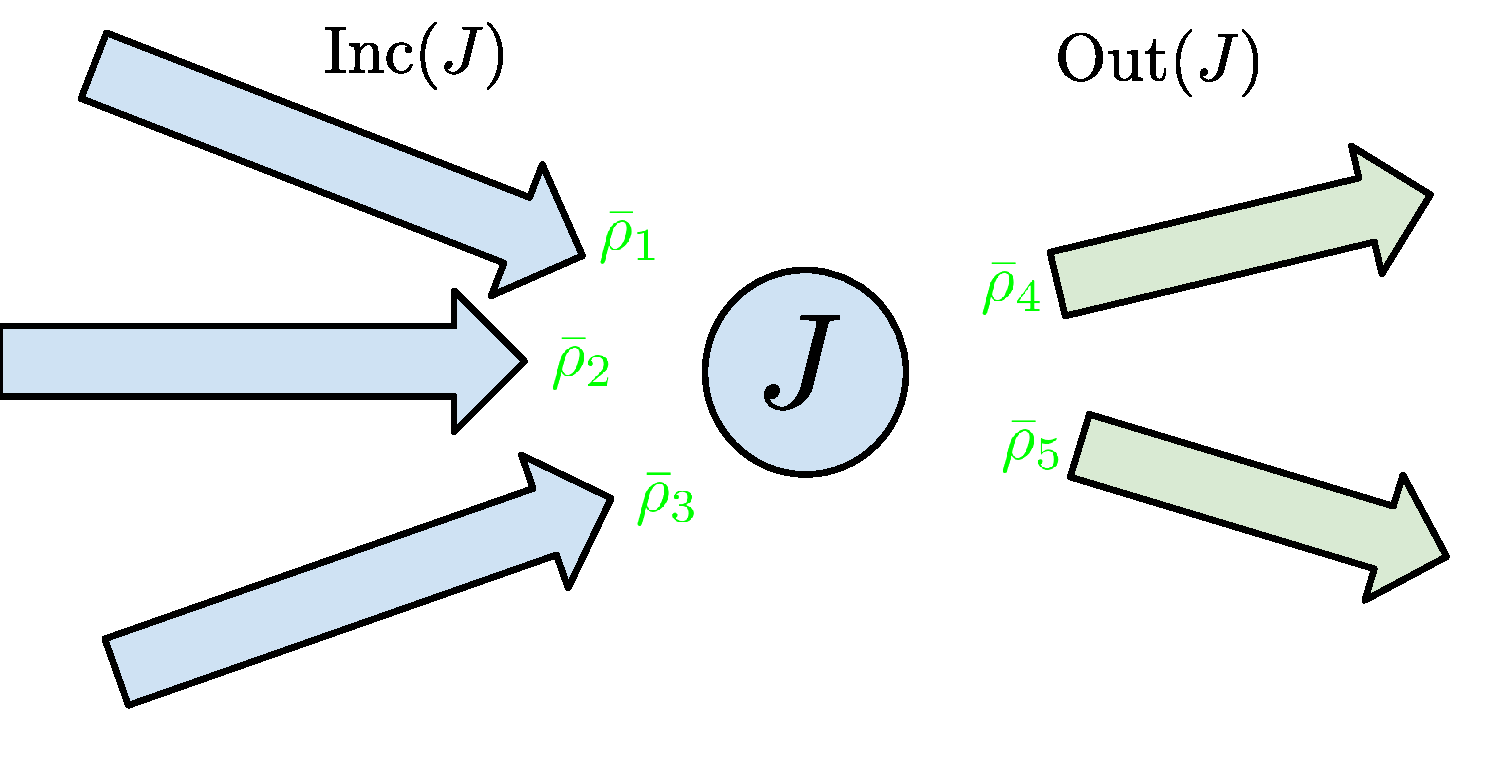
\includegraphics[width=.7\columnwidth]{figs-gen/junctions-riemann}
\end{figure}

\end{frame}

\begin{frame}

Define a \textbf{Riemann Solver} $\RS$:

\begin{align}
\RS:&\mathbb{R}^{m+n}&\rightarrow\mathbb{R}^{m+n}\\&\mathbf{\cvar}_{\jn}^{0}&\mapsto\RS\left(\mathbf{\cvar}_{\jn}^{0}\right)=\hat{\mathbf{\cvar}}_{\jn}
\end{align}

where $\hat{\cvar}^{\link}_{\jn} \in \hat{\mathbf{\cvar}}_{\jn}$ is the boundary condition at the junction interface for link $\link$.

\begin{itemize}
    \item<2-3> Consider a specific link
\end{itemize}

\begin{figure}
\includegraphics<1>[width=.7\columnwidth]{figs-gen/junctions-riemann-rs}
\includegraphics<2>[width=.7\columnwidth]{figs-gen/junctions-riemann-rs-one}
\includegraphics<3>[width=.7\columnwidth]{figs-gen/riemann-junction}
\end{figure}

\end{frame}

\begin{frame}
\frametitle{Conditions on Riemann solver}

\begin{itemize}
    \item<1-> Self-similar
    \begin{equation}\RS\left(\mathbf{\cvar}_{\jn}\right)=\RS\left(\mathbf{\hat{\cvar}}_{\jn}\right)=\mathbf{\hat{\cvar}}_{\jn}\end{equation}
    \item<2-> All shockwaves must emanate outward from junction
    \begin{figure}
    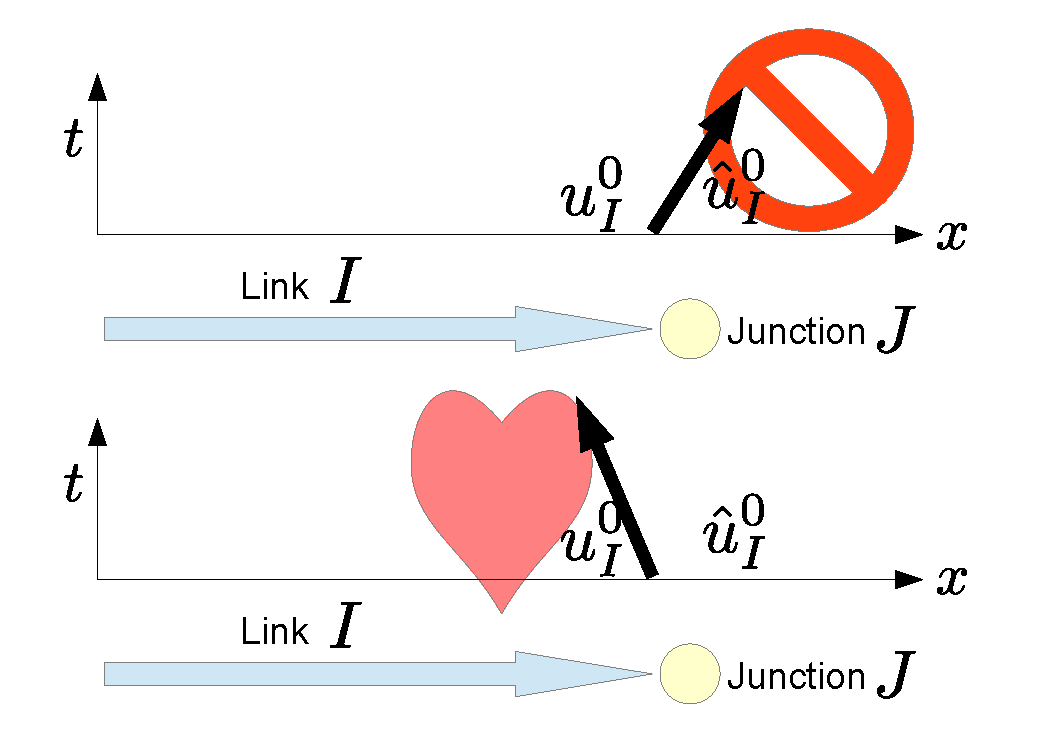
\includegraphics[width=.5\columnwidth]{figs-gen/shock}
    \end{figure}
    \item<3-> Conservation of mass
    \begin{equation}
    \sum_{i\in Inc\left(\jn\right)}f\left(\left\{ \mathbf{\hat{\cvar}}_{\jn}\right\} _{i}\right)=\sum_{j\in Out\left(\jn\right)}f\left(\left\{ \mathbf{\hat{\cvar}}_{\jn}\right\} _{j}\right)
    \end{equation}
\end{itemize}

\end{frame}


\begin{frame}
\frametitle{Riemann solver for linear flux function}
\begin{example}
On board...
\end{example}
\end{frame}
